\chapter{图像处理与特征提取}
\label{chap:rii-image-processing}

\begin{focusbox}{本章复习路线}
从像素出发，先用灰度和邻域运算改善可见性，用几何变换与插值建立像素对应，然后用阈值、边缘或区域法提取目标。对二值掩膜进行形态学处理，再提取尺寸、形状或纹理等特征。\textbf{优先练习}直方图均衡化、双线性插值、滤波与梯度、腐蚀膨胀及开闭运算、OTSU 阈值计算。
\end{focusbox}

本章对应《第4章：图像处理与特征提取》讲义。灰度运算与插值见 PDF 第7--60页，滤波见第61--82页，形态学见第83--97页，分割与缺陷检测见第98--139页。边缘定位、区域面积与测量平面的对应关系见第\ref{chap:rii-image-formation}章。

\section{像素、点运算与直方图}

一幅灰度图可记为 $f(x,y)$，约定 $x$ 为列、$y$ 为行。空间\textbf{采样}决定位置网格的疏密，灰度\textbf{量化}决定幅值的级数。$b$ 位灰度图有 $L=2^b$ 个可用灰度值 $0,\ldots,L-1$。RGB 图像在每个位置记录三分量。亮度描述明暗，反差描述明暗差异，饱和度描述颜色的鲜艳程度。若颜色本身是分类信息，应保留多通道特征。

\dfn{灰度点运算}{对每个输入灰度 $r=f(x,y)$ 使用同一映射，得 $g(x,y)=T[r]$。线性或分段线性拉伸可扩展感兴趣的灰度区间。归一化后令 $0\le r\le1$，伽马变换 $T[r]=r^\gamma$ 在 $0<\gamma<1$ 时提高中间灰度，$\gamma>1$ 时压低中间灰度；对数变换 $T[r]=c\ln(1+r)$ 可展开低灰度区、压缩高灰度区。输出量化时应按题意取整和裁剪。}

\textbf{图像代数与逻辑运算}针对对应像素。例如用乘法或逻辑与保留二值掩膜覆盖的 ROI，用差分观察两幅配准图的变化。多次观测取平均时，若场景保持不变、各帧加性噪声独立且零均值，$M$ 帧平均后噪声方差变为单帧的 $1/M$。计算图像差值前宜转换到有符号或浮点类型。

\subsection{直方图均衡化}

设有 $N$ 个像素，灰度 $k$ 出现 $n_k$ 次。归一化直方图为 $p(k)=n_k/N$，累积分布为 $F(k)=\sum_{i=0}^{k}p(i)$。一种离散均衡化约定为
\[
s_k=\bigl\lfloor (L-1)F(k)\bigr\rfloor .
\]
遍历原图，以 $s_k$ 替代所有灰度为 $k$ 的像素。这个映射保持灰度的非严格次序。离散取整会合并某些灰度级，均衡后的直方图可能仍有峰值。\textbf{直方图规定化}则给出目标分布，按两边的累计概率找最接近的灰度对应关系。

\begin{figure}[htbp]
\centering
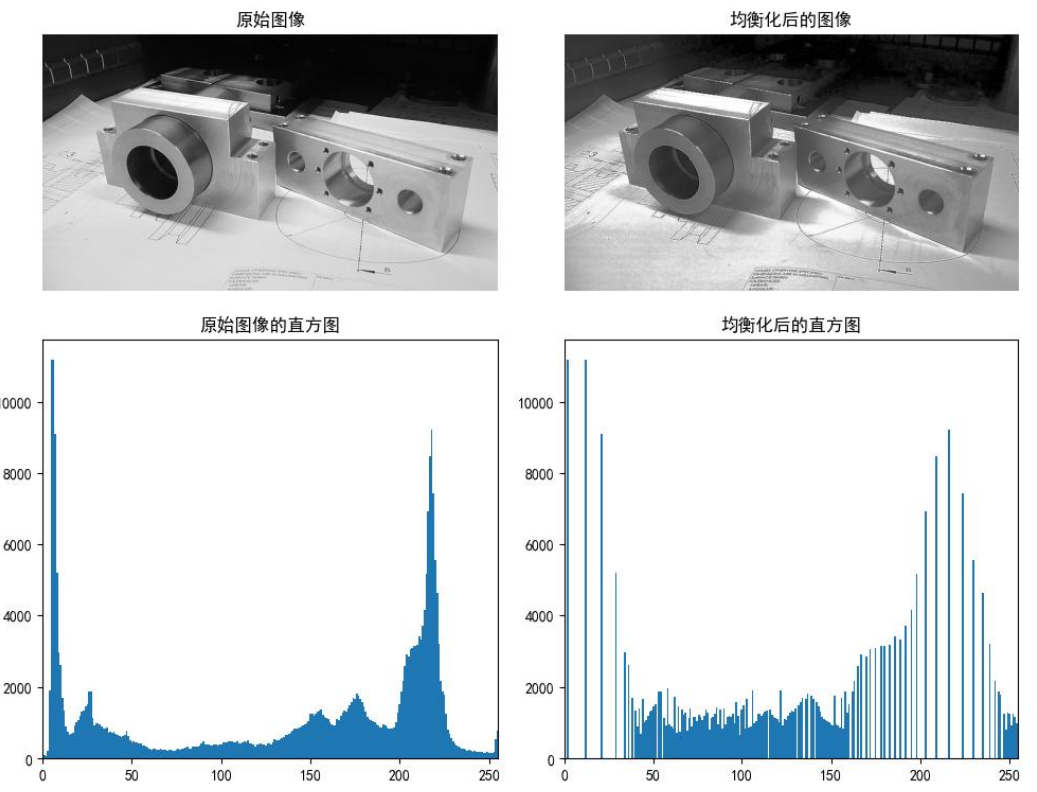
\includegraphics[width=0.75\linewidth]{04-equalization.png}
\caption{均衡化前后的图像和灰度直方图。裁自《第4章：图像处理与特征提取》PDF 第32页。}
\label{fig:rii-hist-equalization}
\end{figure}

\Needspace{5\baselineskip}
\ex{手算四级灰度图的均衡化}{
某 2 位灰度图共 8 像素，灰度 $0,1,2,3$ 的频数分别为 $4,2,1,1$。求按上述向下取整约定得到的映射和输出频数。
\begin{center}
\begin{tabular}{@{}lrrrr@{}}
\toprule
输入灰度 $k$ & $0$ & $1$ & $2$ & $3$ \\
\midrule
$F(k)$ & $4/8$ & $6/8$ & $7/8$ & $8/8$ \\
$(L-1)F(k)$ & $1.5$ & $2.25$ & $2.625$ & $3$ \\
$s_k$ & $1$ & $2$ & $2$ & $3$ \\
\bottomrule
\end{tabular}
\end{center}
输出灰度 $0,1,2,3$ 的频数依次为 $0,4,3,1$，其中输入灰度 1 和 2 都落到输出灰度 2。
}

\nt{有些实现用四舍五入，或先扣除累计分布的最小非零值。手算时先说明取整约定；输出频数要把映射到同一灰度的输入频数相加。直方图只保留各灰度出现次数，仍需位置特征辨别不同形状。}

\section{几何变换和插值}

\subsection{从输出反查输入}

平移、缩放、旋转及剪切可以表示为齐次仿射变换
\[
\begin{bmatrix}x'\\y'\\1\end{bmatrix}
=H\begin{bmatrix}x\\y\\1\end{bmatrix},
\qquad
H=\begin{bmatrix}a&b&t_x\\c&d&t_y\\0&0&1\end{bmatrix}.
\]
若围绕点 $\mathbf c$ 做线性变换 $A$，应使用 $\mathbf p'=A(\mathbf p-\mathbf c)+\mathbf c$。图像的行坐标常向下递增，判断视觉旋转方向时须结合坐标轴方向。
正向变换后取整会使目标网格出现空洞或多点碰撞。对于可逆 $H$，遍历每个输出像素，用 $H^{-1}$ 找其输入坐标，再对原图采样。若反查位置越界，应指定补零、边缘延拓等规则。

\subsection{最近邻、双线性与双三次}

最近邻取离反查位置最近的网格值，适合类别标签。双线性取四个相邻值的加权平均，双三次通常利用 $4\times4$ 邻域，可得到更平滑的结果，代价是计算量更大。图像缩小时，细小结构可能混叠，通常要先适当低通。

\begin{figure}[htbp]
\centering
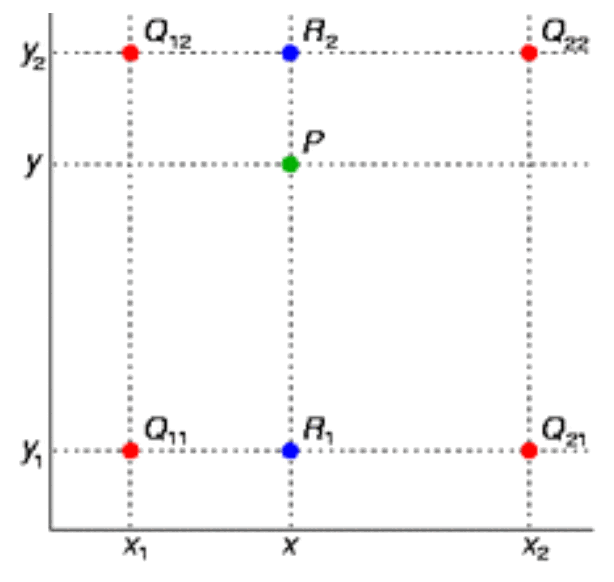
\includegraphics[width=0.45\linewidth]{04-bilinear.png}
\caption{双线性插值的四个网格顶点。先在每一行沿 $x$ 方向插值，再沿 $y$ 方向插值。裁自《第4章：图像处理与特征提取》PDF 第58页。}
\label{fig:rii-bilinear}
\end{figure}

设反查点为 $(i+\alpha,j+\beta)$，$i,j$ 为整数，$0\le\alpha,\beta<1$。先算两行的线性插值
\[
r_0=(1-\alpha)f(i,j)+\alpha f(i+1,j),\qquad
r_1=(1-\alpha)f(i,j+1)+\alpha f(i+1,j+1).
\]
再得 $g=(1-\beta)r_0+\beta r_1$。四个角点权重非负且和为 1，故结果介于这四个值的最小值与最大值之间。

\Needspace{5\baselineskip}
\ex{在反查位置算双线性插值}{
设反查位置为 $(1.25,2.75)$，四个邻点灰度为 $f(1,2)=20$、$f(2,2)=40$、$f(1,3)=60$、$f(2,3)=100$。这里 $\alpha=0.25$、$\beta=0.75$，得
\[
r_0=0.75(20)+0.25(40)=25,\quad r_1=0.75(60)+0.25(100)=70.
\]
所以 $g=0.25(25)+0.75(70)=58.75$。若要求 8 位整数并以四舍五入处理，结果为 59。最近邻选择 $(1,3)$，给出 60。
}

\section{平滑、频域滤波和锐化}

\subsection{空域邻域滤波}

滤波器在滑动窗口内为中心点计算新值。\textbf{均值}等权，\textbf{高斯}让靠近中心的点权重更大，二者都用非负归一化权重，在平坦区域可减弱随机噪声，窗口加大时边缘更易变模糊。高斯核由 $\exp[-(x^2+y^2)/(2\sigma^2)]$ 取样并归一化，$\sigma$ 越大平滑通常越强。\textbf{中值}先排序再取中间值，是非线性滤波；孤立黑白脉冲只要没有占据窗口多数，通常可由它抑制。处理图像边界时应先确定窗口之外的填充规则。

线性邻域运算中，卷积按 $g(x,y)=\sum_{i,j}h(i,j)f(x-i,y-j)$ 相乘求和。若按 $f(x+i,y+j)$ 取邻域，得到相关运算。两者相差一次将核关于中心旋转 $180^\circ$，均值核和中心对称的高斯核旋转后保持原样。手算前应先确认题目约定。

\Needspace{5\baselineskip}
\ex{比较均值、高斯和中值滤波}{
以窗口中心为待更新像素，给定窗口和离散高斯近似核
\[
\begin{bmatrix}20&21&20\\20&255&19\\19&20&20\end{bmatrix},
\qquad
G=\frac1{16}\begin{bmatrix}1&2&1\\2&4&2\\1&2&1\end{bmatrix}.
\]
均值为 $(159+255)/9=46$；用高斯核逐项相乘再相加，得 $(79+160+4\times255)/16=78.6875$；排序为 $19,19,20,20,20,20,20,21,255$，中值为 20。这个窗口的高频异常来自一个孤立亮点，其位置恰在核中心，高斯权重反而让该点对输出影响更大。
}

\subsection{频域滤波与边缘锐化}

令图像横纵尺寸为 $M,N$，二维 DFT 将空间坐标 $(x,y)$ 的信号转换到横纵频率索引 $(u,v)$：
\[
F(u,v)=\sum_{x=0}^{M-1}\sum_{y=0}^{N-1}f(x,y)
\exp\!\left[-2\pi\mathrm{i}\left(\frac{ux}{M}+\frac{vy}{N}\right)\right].
\]
在频域计算 $G=HF$，再作逆 DFT。若频谱经移位使直流位于中心，理想低通取 $H=1$（到中心距离 $D(u,v)\le D_0$）及 $H=0$（$D(u,v)>D_0$）。它能削弱部分高频噪声，同时损失细节。通带边界突变会使空间响应出现振铃。需要用 DFT 实现线性卷积时，还要考虑补零以免引入循环卷积的边界绕回。

\textbf{锐化}可用高频掩模。令 $f_b$ 为平滑图，锐化输出为 $g=f+k(f-f_b)$，其中 $k>0$。也可用四邻接拉普拉斯近似 $\nabla^2f=f_{\text{上}}+f_{\text{下}}+f_{\text{左}}+f_{\text{右}}-4f$，取 $g=f-\lambda\nabla^2f$，$\lambda>0$。若核中心符号反向，回加拉普拉斯响应时的符号也应反向。求梯度或锐化前应留意噪声。

\section{二值图像的形态学}

\subsection{结构元、腐蚀与膨胀}

设 $A$ 是前景为 1 的像素坐标集合，$B$ 为结构元中生效位置相对于锚点的偏移集合。写作 $z+B=\{z+b:b\in B\}$。选好锚点后，用同一坐标约定计算
\[
\begin{aligned}
A\ominus B&=\{z:z+B\subseteq A\},\\
A\oplus B&=\{a+b:a\in A,\ b\in B\}
=\{z:(z+\widehat B)\cap A\ne\varnothing\},\\
\widehat B&=\{-b:b\in B\}.
\end{aligned}
\]
\textbf{腐蚀}可记为“把结构元放到候选锚点，所有有效位置都要落在前景”。\textbf{膨胀}可记为“从每个前景点出发盖出原结构元”，若改为在候选输出点检查是否能碰到输入前景，则使用反射后的结构元 $\widehat B$。对含原点的 $B$，腐蚀缩小或保持前景，膨胀扩大或保持前景。

\subsection{开运算和闭运算}

\[
 A\circ B=(A\ominus B)\oplus B,\qquad
 A\bullet B=(A\oplus B)\ominus B.
\]
开运算先腐蚀后膨胀，可去掉容不下结构元的前景孤点、凸起和细连接；闭运算先膨胀后腐蚀，可填补尺寸和形状与结构元匹配的小裂缝、小空洞，并连接近邻前景。使用同一结构元复做一次开运算或闭运算时，理想集合运算的结果保持不变。

\begin{figure}[htbp]
\centering
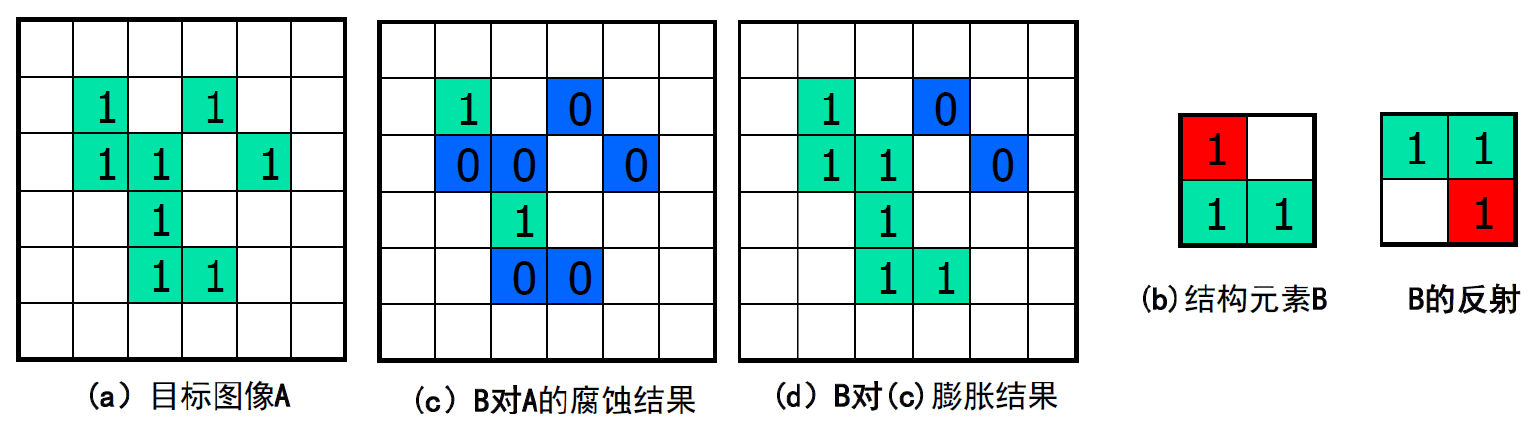
\includegraphics[width=0.96\linewidth]{04-opening.png}
\caption{非对称结构元作用下的开运算。右侧分别为原结构元及其关于锚点的反射。裁自《第4章：图像处理与特征提取》PDF 第95页。}
\label{fig:rii-morph-opening}
\end{figure}

\Needspace{5\baselineskip}
\ex{用集合写出一维开、闭运算}{
取 $A=\{1,2,3,5,6,10\}$，结构元 $B=\{-1,0,1\}$，锚点为 0，窗口在整数线上计算。
\begin{itemize}
\item 只有中心 2 的三个连续位置 $\{1,2,3\}$ 全在 $A$ 中，故 $A\ominus B=\{2\}$。再由中心 2 盖出 $B$，得 $A\circ B=\{1,2,3\}$。
\item 对 $A$ 各点加 $-1,0,1$ 取并集，得 $A\oplus B=\{0,1,\ldots,7\}\cup\{9,10,11\}$。对该集合腐蚀，连续段的两端各退一步，得 $A\bullet B=\{1,2,3,4,5,6,10\}$。
\end{itemize}
开运算去除了短前景段；闭运算补上位置 4，保留了右侧更宽的断开区域。
}

\nt{先看题中前景是黑还是白，再把前景写成集合。结构元的空格不参与覆盖检查。对非对称结构元，若题目要求逐点推膨胀，直接从每个前景位置加 $B$ 通常最方便。}

\section{图像分割：边缘、阈值与区域}

\subsection{梯度边缘与连接}

图像边缘是灰度或纹理在空间上迅速变化的位置。梯度 $\nabla f=(G_x,G_y)^\mathsf T$ 的模 $\sqrt{G_x^2+G_y^2}$ 表示变化强度，角度 $\operatorname{atan2}(G_y,G_x)$ 给出灰度增长最快的方向。在局部直边附近，梯度与边缘切线垂直。实现中也常用 $|G_x|+|G_y|$ 近似强度。对理想阶跃，平滑后在一阶导数幅值的峰附近定位边缘，也可寻找二阶导数的过零点。其他剖面的导数响应见图~\ref{fig:rii-edge-profiles}。

\begin{figure}[htbp]
\centering
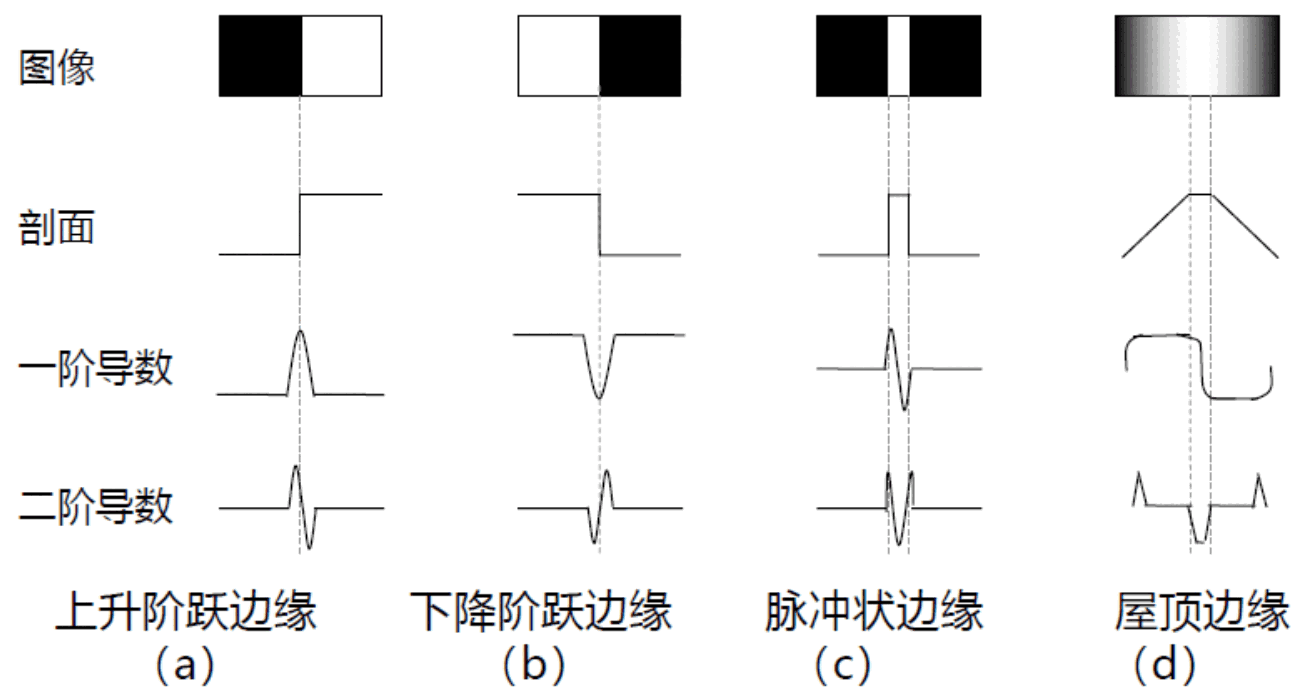
\includegraphics[width=0.86\linewidth]{04-edge-profiles.png}
\caption{四类典型边缘的灰度剖面及导数响应。裁自《第4章：图像处理与特征提取》PDF 第103页。}
\label{fig:rii-edge-profiles}
\end{figure}

以图像的列为 $x$、行为 $y$，若按掩模原顺序与邻域逐项相乘求和（相关），Sobel 算子可取
\[
S_x=\begin{bmatrix}-1&0&1\\-2&0&2\\-1&0&1\end{bmatrix},\qquad
S_y=\begin{bmatrix}-1&-2&-1\\0&0&0\\1&2&1\end{bmatrix}.
\]
Prewitt 用较均匀的横向或纵向平均近似一阶导数，Roberts 在 $2\times2$ 上作对角差分，拉普拉斯给二阶响应。\textbf{Canny}依次做高斯平滑、梯度计算、沿梯度方向非极大值抑制、双阈值与滞后连接，保留与强边缘连通的候选弱边缘。检测得到的边缘可能不连续，若任务为识别几何轮廓，可用 Hough 投票或其他边缘连接方法。

\Needspace{5\baselineskip}
\ex{手算 Sobel 响应并判断边缘方向}{
中心窗口为
$\begin{bmatrix}20&20&80\\20&20&80\\20&20&80\end{bmatrix}$。
按上述掩模，$G_x=(1+2+1)(80-20)=240$，$G_y=0$，梯度模为 240。灰度沿列坐标正向增长，边缘切线沿行坐标方向，对应图像中的竖直边缘。
}

\subsection{全局阈值与 OTSU}

单阈值分割将图像划分为 $f\le t$ 和 $f>t$ 两类，哪一类为前景由任务决定。目标和背景灰度分布分离时，全局阈值计算简单。照明随位置明显变化时，可依据局部窗口统计量设置自适应阈值 $t(x,y)$。

设候选阈值为 $t$，分别计算两类权重 $\omega_0,\omega_1$ 和类均值 $\mu_0,\mu_1$：
\begin{align*}
\omega_0&=\sum_{k=0}^t p(k),& \omega_1&=1-\omega_0,\\
\mu_0&=\frac{\sum_{k=0}^t k p(k)}{\omega_0},&
\mu_1&=\frac{\sum_{k=t+1}^{L-1} k p(k)}{\omega_1}.
\end{align*}
以 $\mu_T=\omega_0\mu_0+\omega_1\mu_1$ 表示整图均值，类间方差为
\[
\sigma_B^2(t)=\omega_0(\mu_0-\mu_T)^2+\omega_1(\mu_1-\mu_T)^2
=\omega_0\omega_1(\mu_0-\mu_1)^2.
\]
\textbf{OTSU（大津法）}枚举使两类皆非空的 $t$，取类间方差最大的阈值。将总平方偏差按类展开，可得总方差等于类内方差与类间方差之和，所以最大化类间方差同时最小化加权类内方差。最佳阈值若并列，应按题意作出取值约定，空灰度段中多个阈值可能对应同一划分。

\Needspace{5\baselineskip}
\ex{给定直方图求 OTSU 阈值}{
设只可能出现灰度 $0,1,2,3$，且每级各有两个像素。枚举 $t=0,1,2$：
\begin{center}
\begin{tabular}{@{}crrrrc@{}}
\toprule
$t$ & $\omega_0$ & $\omega_1$ & $\mu_0$ & $\mu_1$ & $\sigma_B^2$ \\
\midrule
0 & $1/4$ & $3/4$ & $0$ & $2$ & $3/4$ \\
1 & $1/2$ & $1/2$ & $1/2$ & $5/2$ & $1$ \\
2 & $3/4$ & $1/4$ & $1$ & $3$ & $3/4$ \\
\bottomrule
\end{tabular}
\end{center}
例如 $t=1$ 时，低灰度类由 0 和 1 组成，均值 $\mu_0=(0/4+1/4)/(1/2)=1/2$；高类均值同理为 $5/2$。最大类间方差取在 $t=1$，分割为 $\{0,1\}$ 和 $\{2,3\}$。
}

\subsection{区域生长、分裂与合并}

\textbf{区域生长}由种子开始，在四邻域或八邻域中把满足一致性判据的邻点并入区域，直至没有新点可加入。判据可用与种子强度之差，也可用与当前区域均值之差。阈值过小会漏收像素，过大可能穿过边界扩张；种子选择、邻接规则和冲突处理都影响结果。在只沿行列接触的四邻域下，两个角接触的像素各自独立；八邻域中对角接触也算连通。

\textbf{区域分裂与合并}选择区域一致性谓词，例如灰度标准差不超过阈值。用四叉树将不满足条件的块继续分裂，再依据合并判据将相邻且足够相似的区域合并。阈值分割主要看像素强度，边缘分割看突变位置，区域法还使用空间连通性。

\section{缺陷检测与特征分类}

\subsection{从差分图到特征向量}

设待测图为 $I$，无缺陷模板为 $I_0$。固定光照或完成亮度校正，并将两幅图配准后，可令 $D(x,y)=|I(x,y)-I_0(x,y)|$，阈值化得到疑似缺陷。之后用开闭运算清理掩膜，按连通域提取面积、长宽、位置和灰度统计，再按公差筛选。模板错位会在正常轮廓附近生成高差值，因此差分前的配准会直接影响可靠性。

\textbf{特征提取}将图像或感兴趣区域转换为灰度、梯度、几何、直方图或纹理量。\textbf{特征选择}从已有特征中保留有辨别力的分量；若用主成分分析把多维特征投影到低维，新分量由原特征组合而来。在比较单独提取的直方图时，先确认像素数是否需要归一化，再看分布差异；若缺陷判定依赖位置，应结合 ROI、边缘或局部特征。

\subsection{K 近邻与朴素贝叶斯}

\textbf{K 近邻（KNN）}把待判样本与训练样本的特征向量比较，按距离排序，取最近的 $K$ 个样本投票。距离可用欧氏距离 $\bigl[\sum_i(x_i-z_i)^2\bigr]^{1/2}$ 或曼哈顿距离 $\sum_i|x_i-z_i|$。若把面积、长度、灰度等数值尺度不同的量放在同一向量中，应先处理量纲与尺度。$K$ 太小对噪声样本敏感，太大则可能将具有不同性质的样本混入邻居。

\textbf{朴素贝叶斯}由先验概率和类条件似然比较后验。给定特征 $\mathbf x=(x_1,\ldots,x_d)$，在各特征在给定类别 $C$ 时条件独立的假设下，
\[
P(C\mid\mathbf x)\propto P(C)\prod_{j=1}^{d}P(x_j\mid C).
\]
分母 $P(\mathbf x)$ 对各类别相同，分类时比较右侧得分即可。若数据表给的是先验和似然，不能直接把似然当作后验。

\Needspace{9\baselineskip}
\ex{用两项特征判别缺陷}{
设工件缺陷先验为 $0.10$，正常先验为 $0.90$。观察到“面积偏大”和“灰度差偏大”，这两事件在给定类别时条件独立。两事件在缺陷类中的条件概率为 $0.80,0.70$，在正常类中为 $0.10,0.20$。计算类别得分：
\[
s_{\text{缺陷}}=0.10\times0.80\times0.70=0.056,\qquad
s_{\text{正常}}=0.90\times0.10\times0.20=0.018.
\]
故按最大后验概率判缺陷。归一化后缺陷概率为 $0.056/(0.056+0.018)\approx0.757$。
}

\Needspace{8\baselineskip}
\section{公式速查与自测}

\begin{focusbox}{常见题型的第一步}
\textbf{灰度与插值}先确定灰度级数和取整约定，几何题先确定变换方向与像素坐标。\par
\textbf{空间滤波}先写中心窗口，排序取中值或按权重逐项相乘。\par
\textbf{形态学与分割}先明确前景、结构元锚点和邻域，OTSU 要排除空类候选，梯度题分清梯度方向和边缘方向。\par
\textbf{缺陷检测}先保证模板和待测图在位置与亮度上可比，再计算差异和区域特征。
\end{focusbox}

\qs{自测}{
\begin{enumerate}
\item 二值标签图做放大时应优先考虑哪种插值？若是灰度图且希望过渡连续，又可选择什么？
\item 得到一张黑底白字的二值图，白字旁有孤立白点，笔画里有小黑孔。分别可用哪种形态学运算？
\item 对一幅梯度满足 $G_x=0$、$G_y>0$ 的局部图像，边缘走向如何？若图中有高斯噪声，应如何提高梯度的稳定性？
\item 两张图像的灰度直方图完全相同，能否只据此判定工件轮廓一致？用模板做差前应检查什么？
\end{enumerate}
}
\noindent\textbf{核对：}（1）标签用最近邻，灰度图可用双线性。（2）对前景白色用开运算去白点，用闭运算填黑孔，并按尺寸选结构元。（3）梯度沿行坐标正向，边缘沿列坐标方向，求梯度前可作高斯平滑。（4）直方图缺少像素位置信息。应检查配准和照明的一致性。
